%!TEX program = xelatex
\documentclass{beamer}

\usepackage{blindtext}
\usepackage{multicol}

\usetheme{Execushares}

\title{How FOSS can help human to keep their sanity during a pandemic crisis?}
\subtitle{{\it Building better open source projects}}
\author{Pauline Bourmeau (@Ko97551819) - Alexandre Dulaunoy (@adulau)}
\date{June 29, 2020}

\setcounter{showSlideNumbers}{1}

\begin{document}
	\setcounter{showProgressBar}{0}
	\setcounter{showSlideNumbers}{0}

	\frame{\titlepage}

\begin{frame}[fragile]
        \frametitle{Background}
            {\center \it \Large During the lockdown, should we work on an obscure open source natural language processing project\\ or {\bf just do cloth face mask}?\\}
        \begin{flushright}
        Another video chat.
        \end{flushright}
    \end{frame}

\begin{frame}[fragile]
        \frametitle{Meaning of Life}
        \begin{itemize}
                \item {\bf Doing} something which is an imminent and vital need: {\bf face masks\footnote{\url{https://mianmo-project.github.io/}}}
                        \begin{itemize}
                \item It works
                \item and many open source rules and practices apply
                \item What did we learn? and help your next open source security project
                        \end{itemize}
        \end{itemize}
        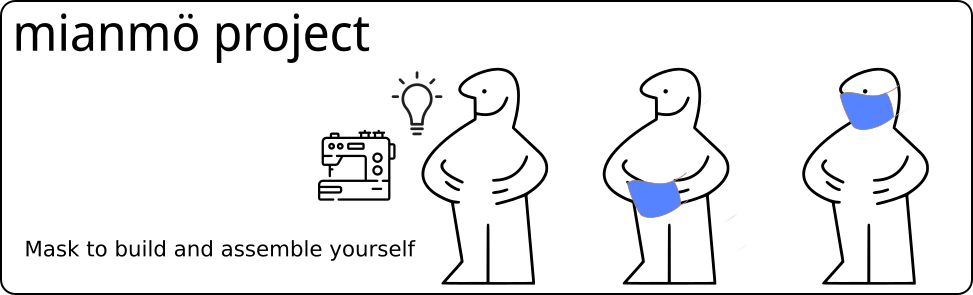
\includegraphics[scale=0.08]{./images/project.png}
    \end{frame}

\begin{frame}[fragile]
        \frametitle{Resonate and be human}

        \begin{multicols}{2}
          \null \vfill
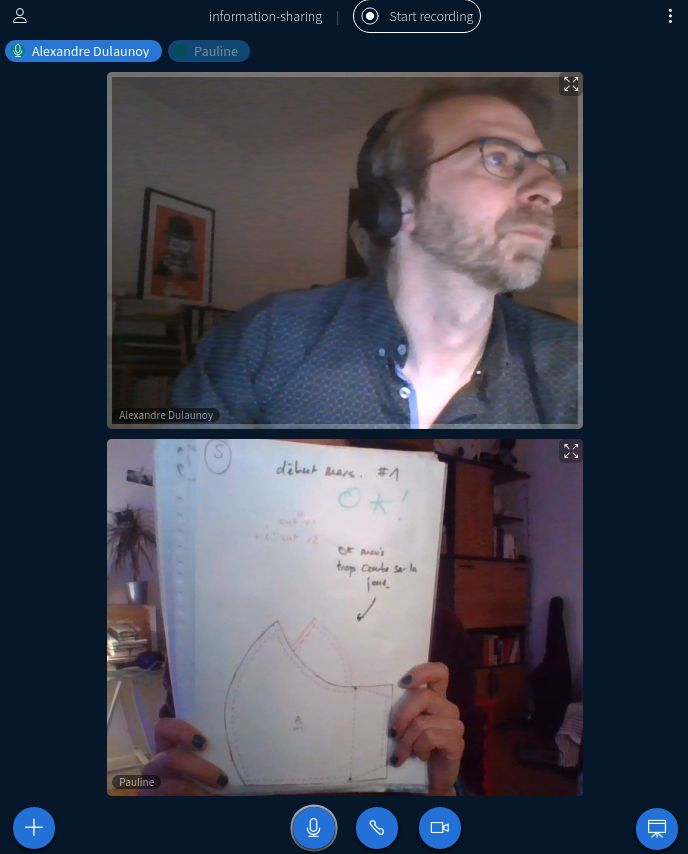
\includegraphics[scale=0.2]{./images/pts-patron-1.png}
  \vfill \null
\columnbreak
           \null \vfill
        \begin{itemize}
                \item {\it Users are wonderful things to have, and not just because they demonstrate that you're serving a need, that you've done something right.}\footnote{The Cathedral and the Bazaar, Eric Steven Raymond}
                \item In other words, face masks without users are useless
                \item {\bf Be your first users}, this will already saves life
        \end{itemize}
          \vfill \null
\end{multicols}
\end{frame}

\begin{frame}[fragile]
        \frametitle{Try and don't be afraid}

        \begin{multicols}{2}
\null \vfill
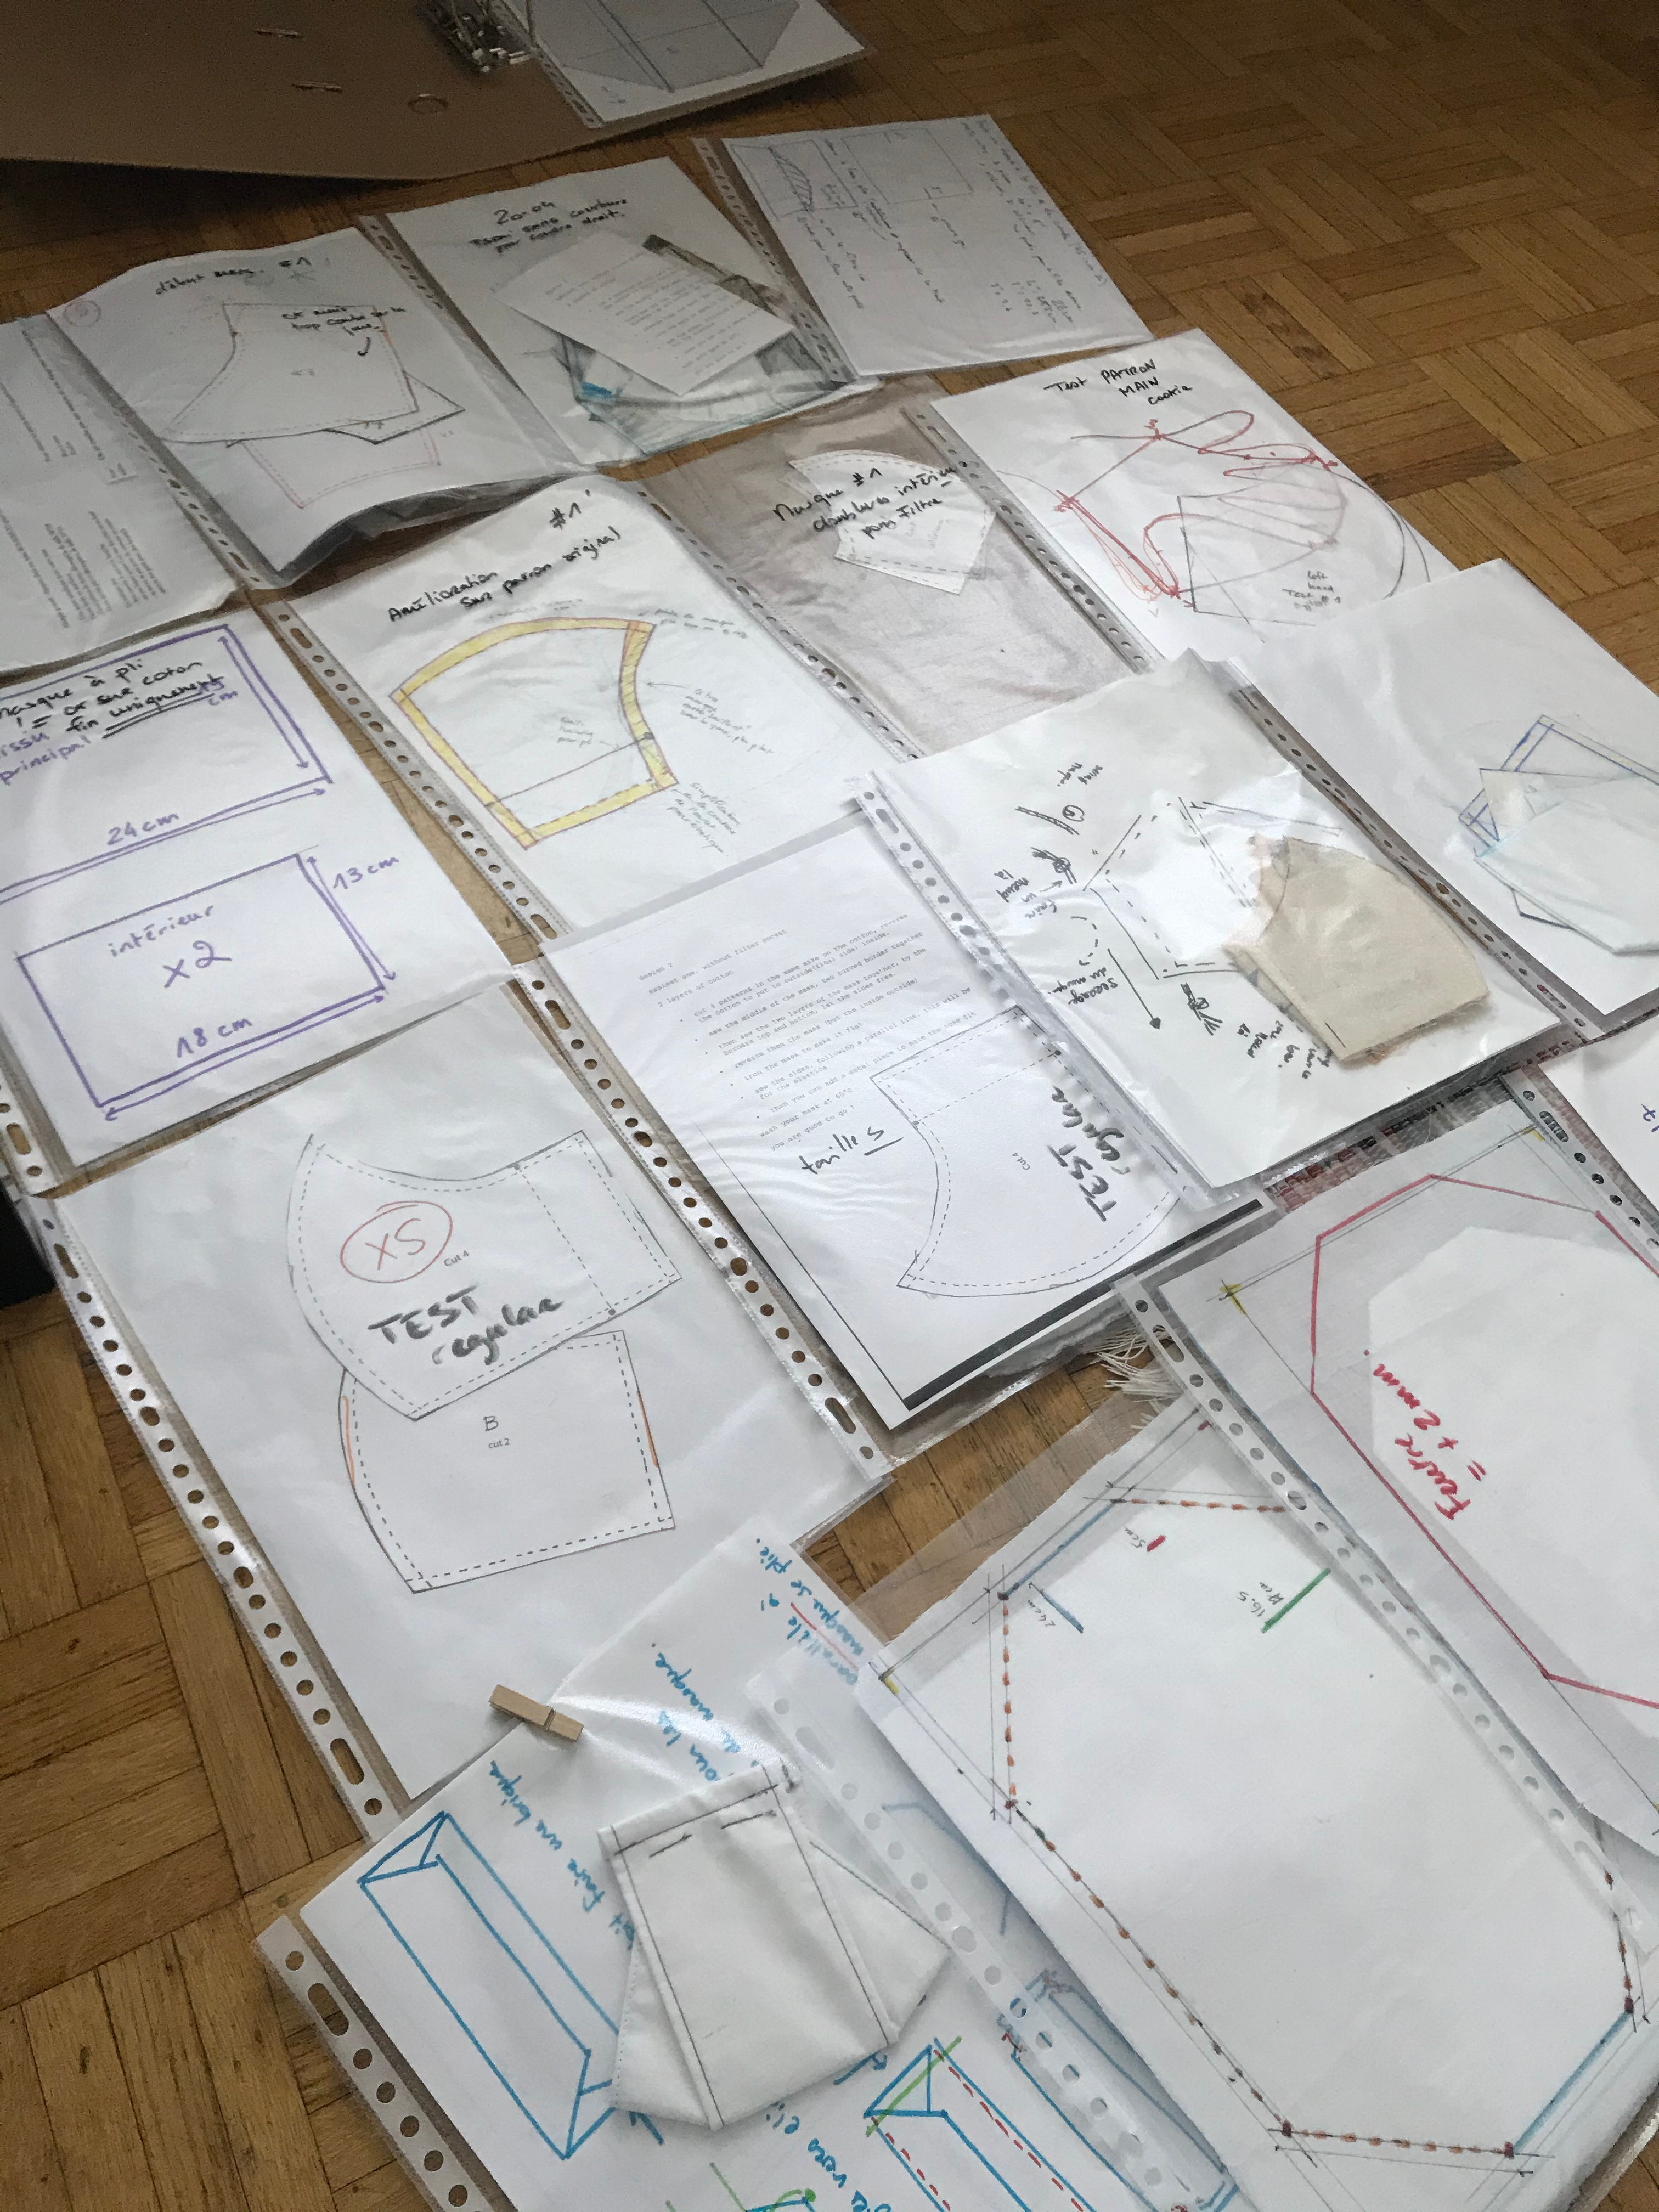
\includegraphics[scale=0.05]{./images/git-log.jpg}
        \vfill \null
        \columnbreak
        \null \vfill
        \begin{itemize}
                \item Learn from scratch
                \item Keep a trace and {\bf publish your failures}
                \item Why git was under-used during the design of cloth face mask?
                \item Keeping track of all face mask design videos is a f*cking challenge\footnote{{\tiny but we enjoyed seeing the different cultures through the lens of face mask design}}
                \item Pick a video and try \footnote{{\tiny bound to YouTube recommendation algorithms}}
                \item Filling the gap of written documentation
        \end{itemize}
         \vfill \null
\end{multicols}
\end{frame}

\begin{frame}[fragile]
        \frametitle{Tooling}
       \begin{multicols}{2}
\null \vfill
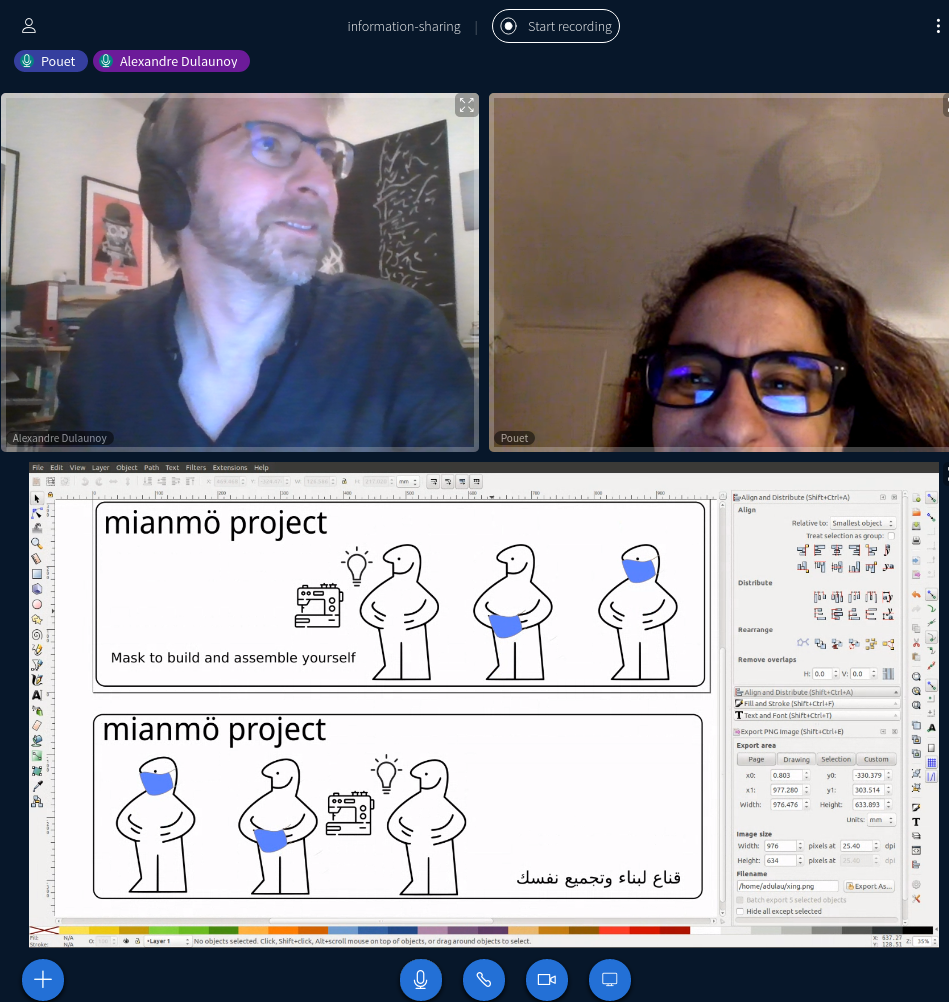
\includegraphics[scale=0.16]{./images/pts-ikea2.png}
       \vfill \null
       \columnbreak
       \null \vfill
       \begin{itemize}
		\item {\it \tiny Ivan Illich defined convivial tools as those most accessible by each person, the least controlled by others, and without restricting equal use by others.}\footnote{Ivan Illich’s book "Tools for Conviviality," published in 1973.}
        \item While designing and building face-masks, people took back the control of the tools by becoming producers
        \item They use the {\bf most easy and accessible tools} (not always open source) to provide guidelines
       \end{itemize}
        \vfill \null
\end{multicols}
\end{frame}

\begin{frame}[fragile]
        \frametitle{Less "Intellectual Property Rights"}
        \begin{itemize}
        \item The fluidity of creative exchanges was helped by fewer legal constraints
        \item Social pressure can help in such period
        \item Many projects during the lock-down relied on {\bf existing open source, free software and content licensing schemes}
        \item A lot of cloth face mask designers didn't know they were doing open source
        \end{itemize}

\end{frame}

\begin{frame}[fragile]
        \frametitle{Reinforcing Social Relationships}
        \begin{multicols}{2}
        \null \vfill
        
\includegraphics[scale=0.08]{./images/soutif.png}
        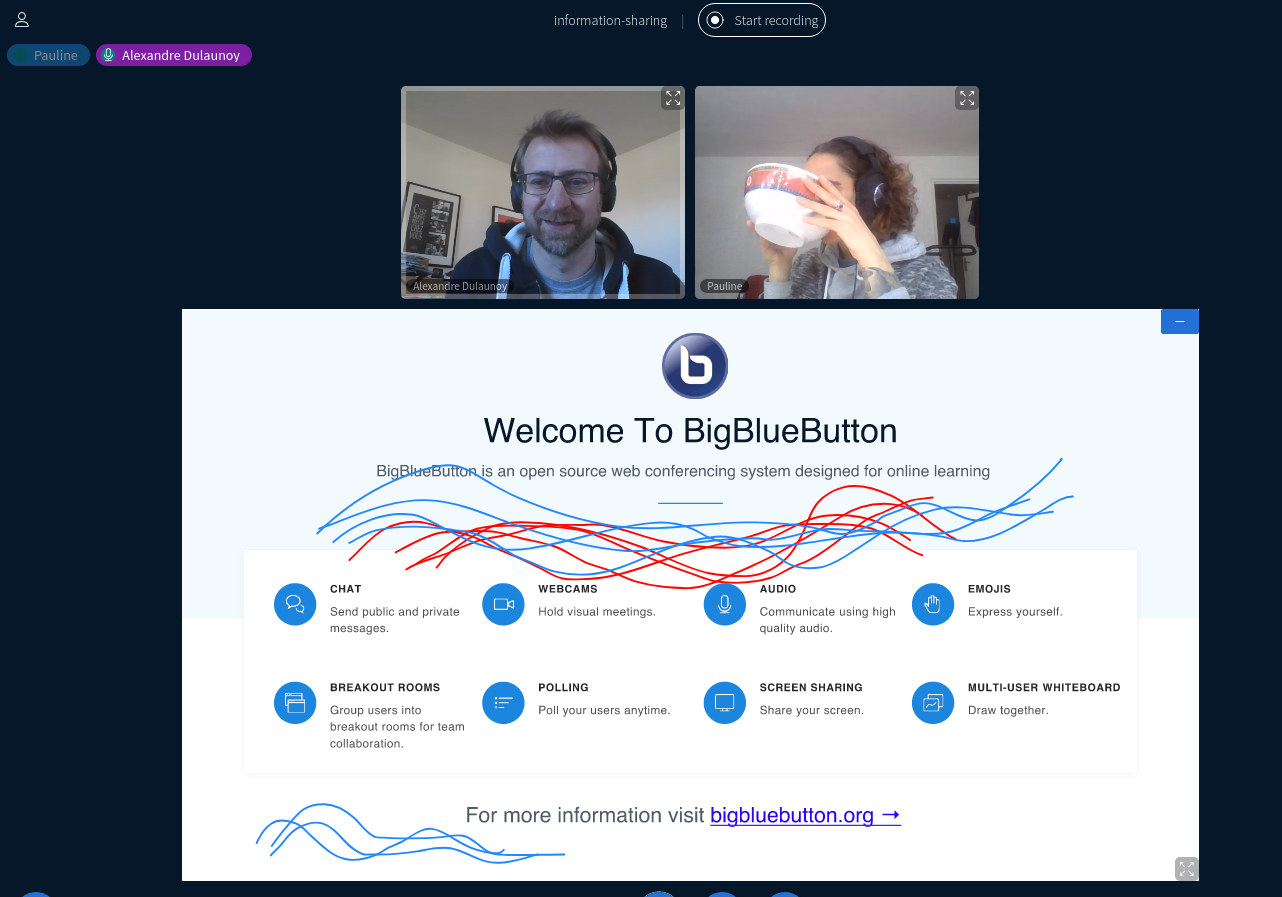
\includegraphics[scale=0.08]{./images/miso.png}
        \vfill \null
        \columnbreak
        \null \vfill
        \begin{itemize}
                \item {\bf Fun is key} to keep sanity in an open source community
          \item With covid-19, all open source contributors discovered the social reality of existing remote contributors
          \item Relying on the existing experience of managing open source community\footnote{Social Architecture - Building On-line Communities by Pieter Hintjens}
        \end{itemize}
        \vfill \null
        \end{multicols}
\end{frame}

\begin{frame}[fragile]
        \frametitle{Fun is really important}
        
\includegraphics[scale=0.2]{./images/boite.png}
\end{frame}

\begin{frame}
        \frametitle{How to cultivate your FOSS project?}
        \begin{itemize}
                \item Fun is important but the gift aspect is a strong community cement
                \item Sharing common tools and objectives to create values
                \item Create knowledge via open source projects as a medium
                \item {\bf Reciprocity to support self-management of open source communities}
                \item Diverse contributors and contribution ensure project stability
        \end{itemize}
\end{frame}

\begin{frame}[fragile]
        \frametitle{Thank You}
        \begin{itemize}
                \item {\bf Markdown} format and all the open source rendering implementations
                \item {\bf Inkscape} (to make cool logos for open source project)
                \item {\bf git} (even if the handling of binary files is still hard)
                \item {\bf BBB BigBlueButton} and {\bf Jitsi} (diversity is good when one fails)
                \item {\bf Python} (for extracting large table of filtering tests only available in crappy PDF generated from an unpublished XLS file)
                \item {\bf SciHub} (thanks Alexandra) as it was the only way to download the academic papers about the filtering of textile fabrics
                \item {\bf All the people who did face masks} and didn't know they were part of the open source and maker community
        \end{itemize}
\end{frame}


\begin{frame}[fragile]
        \frametitle{Where We Succeeded}
        \begin{itemize}
                \item The {\bf open source and maker communities resonated} during the crisis with a lot of initiatives
                \item The past 20+ years of open source licensing did help a lot (less friction in exchange)
                \item Git repositories supported the coordination effort on contributions and content publishing
        \end{itemize}
\end{frame}

\begin{frame}[fragile]
        \frametitle{Where We Failed}
        \begin{itemize}
                \item Some open source tools are still {\bf too complex} to use compared of the sharing of a YouTube video
                \item We are still bad at indexing, evaluating, coordinating and archiving projects (how many face mask designs on GitHub?)
                \item Release early, release often. We failed there as early was a matter of days and not weeks
                \item {\bf Opportunity for new open source projects} such as markdown notes taking and video screenshot at the same time
        \end{itemize}
\end{frame}

\appendix
	\backupbegin
	  \begin{frame}
	    \frametitle{Bibliography}
        \begin{enumerate}
                \item Ivan Illich, Tools for Conviviality, 1973. {\tiny \url{https://co-munity.net/system/files/ILLICH\%201973\_tools\_for\_convivality\_1.pdf}}
                \item Eric Steven Raymond, The Cathedral and the Bazaar, 1997. {\tiny \url{http://www.catb.org/~esr/writings/cathedral-bazaar/}}
                \item Pekka Himanen, The Hacker Ethic, 2001.
                \item Pieter Hintjens, Social Architecture - Building On-line Communities, 2016. {\tiny \url{http://www.foo.be/docs-free/social-architecture/book.pdf}}
        \end{enumerate}
	  \end{frame}
	\backupend

\end{document}
